\documentclass[journal]{IEEEtran}
\usepackage[a5paper, margin=10mm]{geometry}
%\usepackage{lmodern} % Ensure lmodern is loaded for pdflatex
\usepackage{tfrupee} % Include tfrupee package


\setlength{\headheight}{1cm} % Set the height of the header box
\setlength{\headsep}{0mm}     % Set the distance between the header box and the top of the text


%\usepackage[a5paper, top=10mm, bottom=10mm, left=10mm, right=10mm]{geometry}

%
\setlength{\intextsep}{10pt} % Space between text and floats

\makeindex


\usepackage{cite}
\usepackage{amsmath,amssymb,amsfonts,amsthm}
\usepackage{algorithmic}
\usepackage{graphicx}
\usepackage{textcomp}
\usepackage{xcolor}
\usepackage{txfonts}
\usepackage{listings}
\usepackage{enumitem}
\usepackage{mathtools}
\usepackage{gensymb}
\usepackage{comment}
\usepackage[breaklinks=true]{hyperref}
\usepackage{tkz-euclide} 
\usepackage{listings}
\usepackage{multicol}
\usepackage{xparse}
\usepackage{gvv}
%\def\inputGnumericTable{}                                 
\usepackage[latin1]{inputenc}                                
\usepackage{color}                                            
\usepackage{array}                                            
\usepackage{longtable}                                       
\usepackage{calc}                                             
\usepackage{multirow}                                         
\usepackage{hhline}                                           
\usepackage{ifthen}                                               
\usepackage{lscape}
\usepackage{tabularx}
\usepackage{array}
\usepackage{float}
\usepackage{ar}
\usepackage[version=4]{mhchem}


\newtheorem{theorem}{Theorem}[section]
\newtheorem{problem}{Problem}
\newtheorem{proposition}{Proposition}[section]
\newtheorem{lemma}{Lemma}[section]
\newtheorem{corollary}[theorem]{Corollary}
\newtheorem{example}{Example}[section]
\newtheorem{definition}[problem]{Definition}
\newcommand{\BEQA}{\begin{eqnarray}}
\newcommand{\EEQA}{\end{eqnarray}}

\theoremstyle{remark}


\begin{document}
\bibliographystyle{IEEEtran}
\onecolumn

\title{2.8.12}
\author{Josyula G S Avaneesh- EE25BTECH11030}
\maketitle


\renewcommand{\thefigure}{\theenumi}
\renewcommand{\thetable}{\theenumi}
\textbf{Question} Show that the tangent of an angle between the lines
$$\frac{x}{a}+\frac{y}{b}=1$$
$$\frac{x}{a}-\frac{y}{b}=1$$
is $\dfrac{2ab}{a^2-b^2}$\\
\textbf{Solution :} Given details:
\begin{align}
   \myvec{\dfrac{1}{a}&&\dfrac{1}{b}}\vec{x}=1\\
   \myvec{\dfrac{1}{a}&&\dfrac{-1}{b}}\vec{x}=1
\end{align}
\textbf{Property:} The cosine of the angle between line 1 and line 2 is given by $\dfrac{{n_1}^\top n_2}{\norm{n_1}\norm{n_2}} $.

Let the angle between the lines be $\theta$.
\begin{align}
   \cos\theta=\dfrac{{\myvec{\frac{1}{a}&&\frac{1}{b}}}^\top \myvec{\frac{1}{a} && \frac{-1}{b}}}{{\norm{\myvec{\frac{1}{a}&&\frac{1}{b}}}}\norm{\myvec{\frac{1}{a}&&\frac{-1}{b}}}}\\
   \cos\theta=\frac{\frac{1}{a^2}-\frac{1}{b^2}}{\sqrt{\brak{{\frac{1}{a}}^2}+\brak{\frac{1}{b}}^2}\sqrt{\brak{{\frac{1}{a}}^2}+\brak{\frac{-1}{b}}^2}}\\
   \cos\theta=\frac{b^2-a^2}{a^2+b^2}
   \brak{\because \tan\theta=\frac{\sqrt{1-\cos^2\theta}}{\cos\theta}}\\
   \tan\theta=\left|\frac{2ab}{b^2-a^2}\right|
\end{align}
$\therefore$ The tan of the acute angle between the lines is $\dfrac{2ab}{a^2-b^2}$.
\begin{figure}[H]
    \centering
    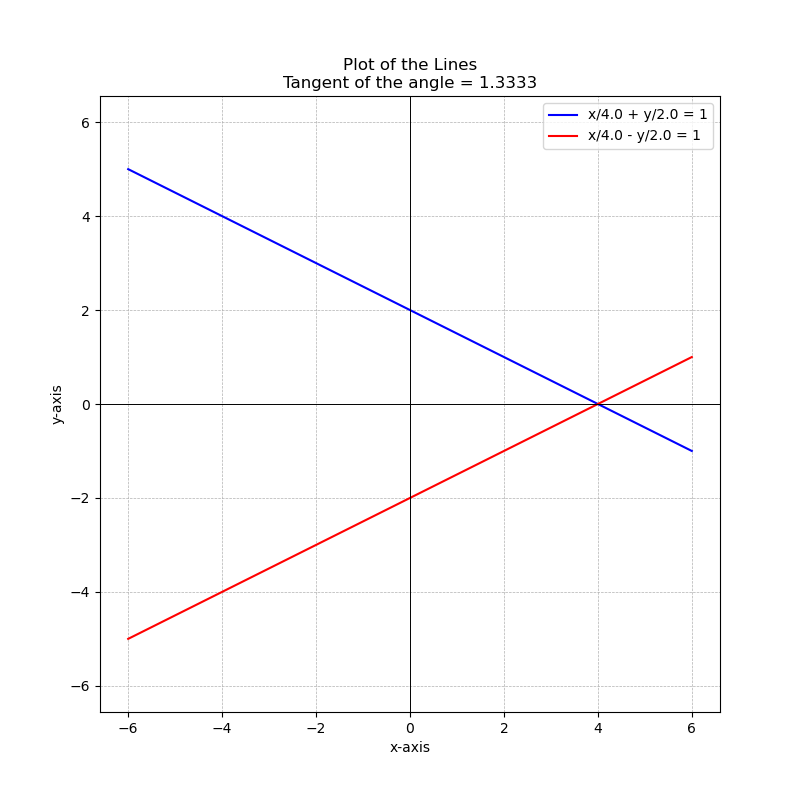
\includegraphics[width=1\columnwidth]{figs/line.png}
    \caption{Plot of the lines}
    \label{fig:placeholder_1}
\end{figure}

\end{document}